% ----------------------------------------------------------------------
%  Pracovní úkoly
% ----------------------------------------------------------------------
\section{Pracovní úkoly}

\begin{enumerate}
\item Určete závislost povrchového napětí \(\sigma\) na objemové koncentraci \(c\) roztoku etylalkoholu ve vodě odtrhávací metodou.

\item Sestrojte graf této závislosti.

\end{enumerate}

% ----------------------------------------------------------------------
%  Teoretická část
% ----------------------------------------------------------------------
\section{Teoretická část}

Povrchovým napětím \(\sigma\) nazýváme kolmou sílu působící na jednotkovou délku na povrch určité látky. Zároveň je tato síla stejná ve všech místech povrchu. Povrchovým napětím se zabýváme zejména u kapalin. Velikost napětí je závislá na teplotě a čistotě kapalin. Látky, které ovlivňují tuto hodnotu, se nazývají povrchově aktivní.

Závislost povrchového napětí na koncentraci budeme měřit tzv. odtrhávací metodou. K měření použijeme torzní váhy, jejichž schéma je znázorněno na obrázku \ref{fig:torzni-vahy}.

\begin{figure}[h]
    \centering
    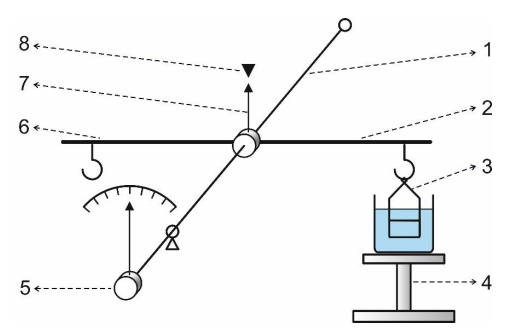
\includegraphics[width=0.5\linewidth]{4 - Závislost povrchového napětí na koncentraci povrchově aktivní látky//Protokol_povrchové napětí//img/Schéma torzních vah.png}
    \caption{Schéma torzních vah}
    \label{fig:torzni-vahy}
\end{figure}

Na pravé straně vah je umístěna nádoba se zkoumanou kapalinou. Do ní je ponořen trámek (3). Na levé straně (6) je umístěno závaží tak, aby byly váhy vyváženy. Nádoba je postupně posouvána dolů (4) a váhy jsou zároveň vyvažovány tak, aby šipka (7) mířila stále na ukazatel (8). V určitý moment je povrchové napětí překonáno a trámek povyskočí směrem vzhůru. V tuto chvíli je zastaveno posouvání a je zaznamenán rozdíl hmotností během zatěžování. Odtud můžeme určit sílu \(P_0\) potřebnou k odtržení trámku.

\begin{equation}
    P_0 = (m_1 - m_2) \cdot g
\end{equation}

kde \(m_1\) a \(m_2\) je počáteční a konečná hmotnost torzních vah a \(g\) gravitační zrychlení. Drátek trámku je je při vytahování z kapaliny držen silou

\begin{equation}
    2F = 2 \sigma \cdot l
\end{equation}

kde \(l\) je délka drátu.

Síla \(P_0\) odpovídá síle \(2F\) a proto dostáváme vztah pro povrchové napětí

\begin{equation}
    \sigma = \frac{(m_1 - m_2)\cdot g}{2l}
\end{equation}

a tedy

\begin{equation}
    \sigma = \frac{P_0}{2l}
\end{equation}

Pro přesnější určení povrchového napětí s korekcí tloušťky drátu použijeme

\begin{equation}
    \sigma_k = \frac{P_2 - P_1}{2l}-r\Bigg(\sqrt{\frac{(P_2 - P_1)\rho g}{l}}-\frac{P_2 - P_1}{l^2} \Bigg)
\end{equation}

kde \(\rho\) je hustota drátu a \(r\) je poloměr drátu.

% ----------------------------------------------------------------------
%  Výsledky a zpracování měření
% ----------------------------------------------------------------------
\section{Výsledky a zpracování měření}

\subsection{Laboratorní podmínky}

    Měření bylo prováděno za laboratorních podmínek uvedených v tabulce \ref{tab:lab_pod}.

    \begin{table}[h]
        \centering
        \begin{tabular}{|c|c|c|} 
        \hline
            t / °C & p / hPa & vlhkost / \%RH  \\ 
        \hline
            24,0(4)   & 989,2(20)   & 42,0(25)            \\
        \hline
        \end{tabular}
        \caption{Laboratorní podmínky}
        \label{tab:lab_pod}
    \end{table}

\subsection{Měření povrchového napětí}

Na začátku bylo třeba důkladně vyčistit lihem a destilovanou vodou část aparatury, abychom zamezily ovlivněni výsledků nečistotami. Dále jsme změřili základní rozměry. Průměr drátu $d$ v rámečku byl změřen třikrát na různých místech se stejnou hodnotou, není tedy třeba počítat aritmetický průměr a směrodatné odchylky. Šířka rámečku $l$ byla spočtena jako aritmetický průměr ze dvou naměřených hodnot se směrodatnou odchylkou uvedených v tabulce \ref{tab:zakladni-rozmery}. Uvedená chyba je rovna součtu druhých mocnin pod odmocninou chyby měřidla a směrodatné odchylky. Vzdálenost $d$ byla měřena mikrometrem s chybou 0,01 mm a délka $l$ posuvným měřidlem s chybou 0,05 mm.

\begin{table}[h]
\centering
\begin{tabular}{|c|ccc|cc|}
\hline
d / mm & 0,79 & 0,79  & 0,79 & 0,79  & \pm 0,010     \\ \hline
l / cm & 2,1  & 2,075 &      & 2,085 & \pm 0,014 \\ \hline
\end{tabular}
\caption{Tabulka základních rozměrů}
\label{tab:zakladni-rozmery}
\end{table}

Roztok v poměru 1:1 jsme vytvořili smícháním jednoho dílu vody a lihu. Přidáním jednoho dílu tohoto roztoku k jednomu dílu destilované vody jsme získali poměr 2:1, dále potom 4:1 atd. Zvolili jsme přidávání vody, protože po změření čisté vody, lihu a poměru 1:1 se vetší rozptyl hodnot nacházel mezi 0\% a 50\% lihu v destilované vodě, proto dává smysl zabývat se tímto intervalem. U každého připraveného vzorku byla zvážena hmotnost pyknometrem, tedy při stejném objemu. Dále byla změřena teplota, protože se jedné o exotermickou reakci během přípravy. Tato teplota byla ve vodní lázni ochlazena na teplotu okolí.

Chyba byla odhadnuta pomocí metody přenosu chyb jako

\begin{equation}
    \sigma_{\sigma} = \frac{1}{2}\sqrt{\frac{l^2 \sigma^2_{P_0}+P^2_0 \sigma^2_l}{l^4}}
\end{equation}

Chyba $\sigma_{m_0} = 3 $ mg, odtud $\sigma_{P_0} = 9,81 \cdot \sigma_{m_0}$. Povrchové napětí $\sigma_k$ je spočtena podle (5). Pro tento výpočet byly použity hustotu změřené pro každý vzorek, uvedených v tabulce \ref{tab:hustoty}. Chyba $\sigma_{\sigma_k}$ byla spočtena jako stejná relativní chyba napětí bez korekce průměru drátu. Za konstantu $g = 9,81 \; m \cdot s^{-2}$ je dosazeno podle [4]. Informativně jsou v tabulce \ref{tab:teplota-smichani} uvedeny teploty, ze kterých bylo vzorek třeba ochladit, po smíchání obou látek. Graf \ref{fig:zavislost-napeti} zobrazuje závislost povrchového napětí na koncentraci lihu ve vodě s korekcí a bez. Dále jsou tyto závislosti nafitovány exponenciální křivkou, jejichž parametry jsou zde také uvedeny.

\begin{table}[h]
\centering
\begin{tabular}{|cccccccc|}
\hline
\multicolumn{1}{|c|}{Poměr destil. voda : líh} &
  \multicolumn{1}{c|}{P_0 / N} &
  \multicolumn{1}{c|}{\sigma / 10^{-3} N \cdot m^{-1}} &
  \multicolumn{1}{c|}{\overline{\sigma}} &
  \multicolumn{1}{c|}{\sigma_{\sigma} / 10^{-3} N \cdot m^{-1}} &
  \multicolumn{1}{c|}{{\sigma_k / N \cdot m^{-1}}} &
  \multicolumn{1}{c|}{\overline{\sigma_k} / 10^{-3} N \cdot m^{-1}} &
  \sigma_{\sigma_k} \\ \hline
1:0  & 0,0032 & 80,93 & 83,22 & 0,89 & 0,065 & 67,32 & 0,74 \\
     & 0,0034 & 84,86 &       & 0,90 & 0,069 &       & 0,72 \\
     & 0,0034 & 83,88 &       & 0,90 & 0,068 &       & 0,72 \\ \hline
0:1  & 0,0014 & 33,84 & 34,17 & 0,75 & 0,025 & 25,10 & 0,56 \\
     & 0,0014 & 34,09 &       & 0,75 & 0,025 &       & 0,55 \\
     & 0,0014 & 34,58 &       & 0,75 & 0,025 &       & 0,55 \\ \hline
1:1  & 0,0016 & 39,73 & 41,53 & 0,76 & 0,029 & 30,82 & 0,59 \\
     & 0,0017 & 42,67 &       & 0,77 & 0,032 &       & 0,56 \\
     & 0,0017 & 42,18 &       & 0,77 & 0,031 &       & 0,56 \\ \hline
3:1  & 0,0022 & 54,69 & 54,36 & 0,80 & 0,042 & 41,77 & 0,61 \\
     & 0,0022 & 54,94 &       & 0,80 & 0,042 &       & 0,61 \\
     & 0,0021 & 53,46 &       & 0,80 & 0,041 &       & 0,62 \\ \hline
7:1  & 0,0027 & 67,93 & 67,28 & 0,84 & 0,054 & 53,09 & 0,66 \\
     & 0,0026 & 66,22 &       & 0,84 & 0,052 &       & 0,67 \\
     & 0,0027 & 67,69 &       & 0,84 & 0,053 &       & 0,66 \\ \hline
15:1 & 0,0031 & 76,27 & 76,19 & 0,87 & 0,061 & 61,06 & 0,70 \\
     & 0,0030 & 75,78 &       & 0,87 & 0,061 &       & 0,70 \\
     & 0,0031 & 76,52 &       & 0,87 & 0,061 &       & 0,70 \\ \hline
\end{tabular}
\caption{Povrchové napětí}
\label{tab:povrchove-napeti}
\end{table}

\begin{table}[h]
\centering
\begin{tabular}{|c|c|c|c|}
\hline
Poměr destil. voda : líh & Objem / ml & Hmotnost / g & Hustota / kg \cdot m^3 \\ \hline
1:0                      & 25         & 24,7         & 988                    \\ \hline
0:1                      & 25         & 19,84        & 793,6                  \\ \hline
1:1                      & 25         & 22,73        & 909,2                  \\ \hline
3:1                      & 25         & 23,91        & 956,4                  \\ \hline
7:1                      & 25         & 24,41        & 976,4                  \\ \hline
15:1                     & 25         & 24,45        & 978                    \\ \hline
\end{tabular}
\caption{Hustota různých vzorků}
\label{tab:hustoty}
\end{table}

\begin{table}[h]
\centering
\begin{tabular}{|c|c|}
\hline
Poměr destil. voda : líh & Teplota / °C \\ \hline
1:0                      & 23,4         \\ \hline
0:1                      & 23,5         \\ \hline
1:1                      & 29           \\ \hline
3:1                      & 26,8         \\ \hline
7:1                      & 24,6         \\ \hline
15:1                     & 23,6         \\ \hline
\end{tabular}
\caption{Teplota vzorku po smíchání}
\label{tab:teplota-smichani}
\end{table}

\begin{figure}[H]
    \centering
    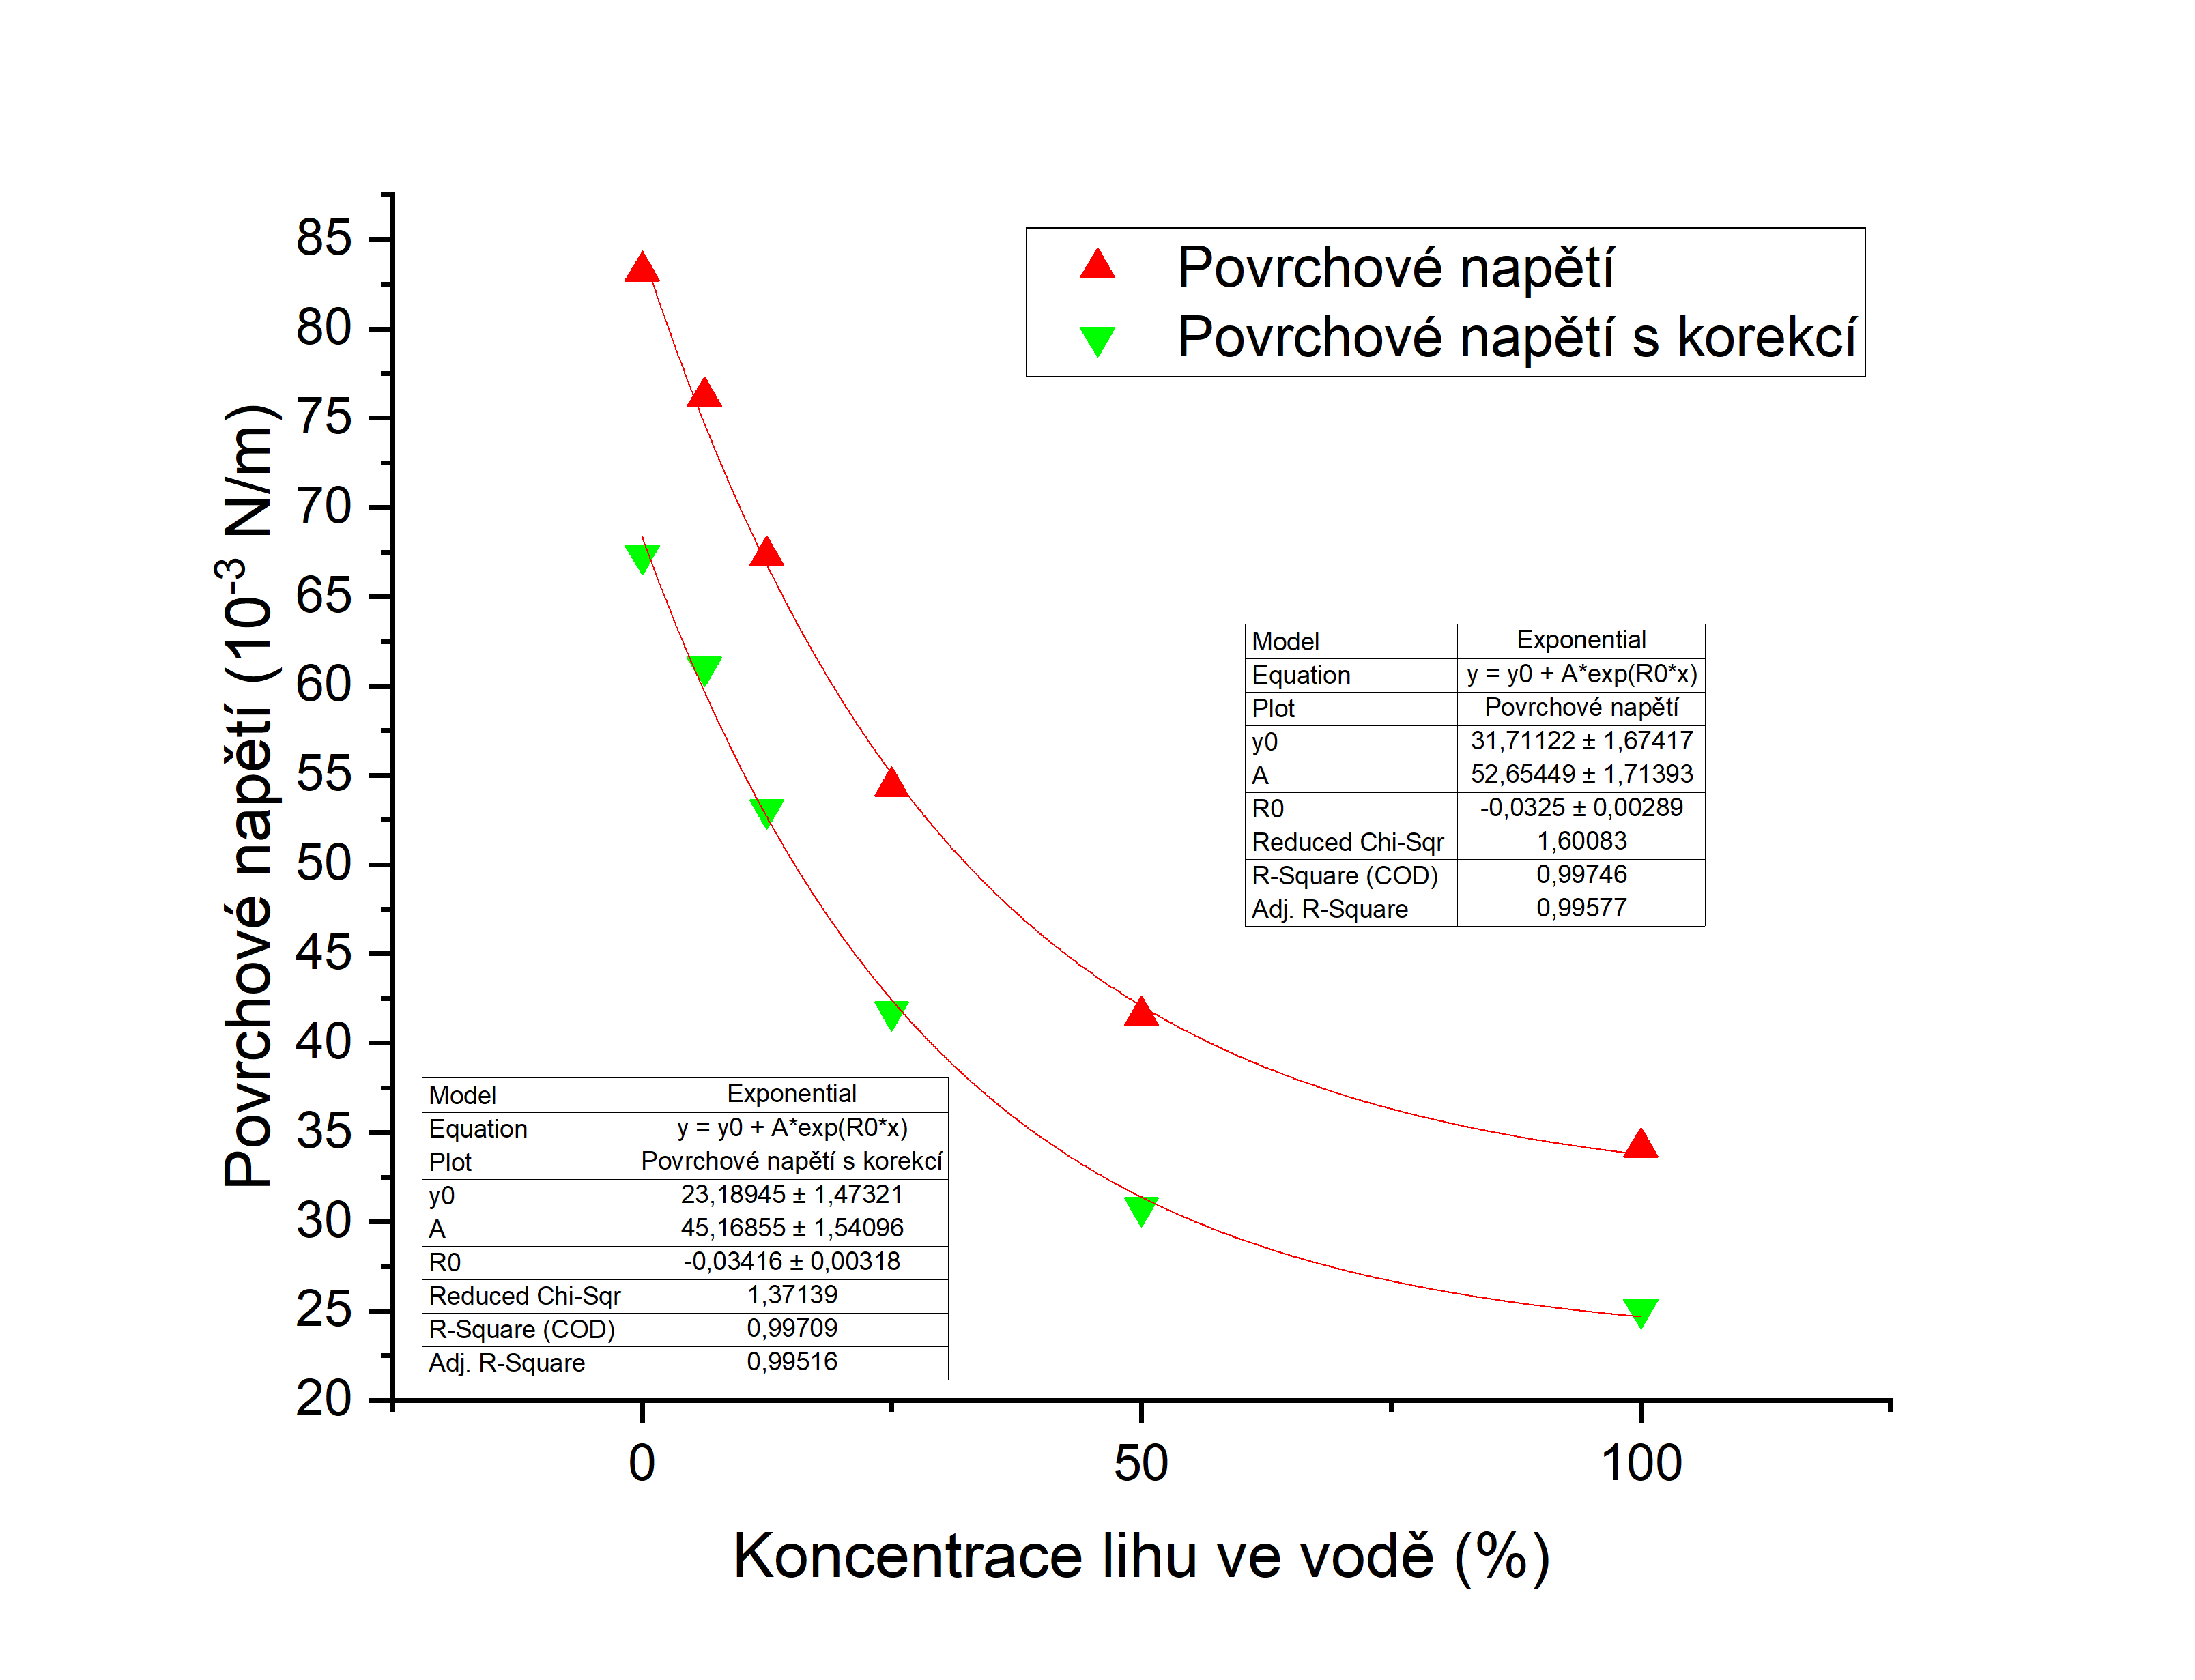
\includegraphics[width=1\linewidth]{4 - Závislost povrchového napětí na koncentraci povrchově aktivní látky//Protokol_povrchové napětí//img/Závislost povrchového napětí na koncentraci.png}
    \caption{Závislost povrchového napětí na koncentraci látky}
    \label{fig:zavislost-napeti}
\end{figure}

\newpage

Nakonec jsme změřili jakou silou je rámeček nadnášen v klidu. Jedná se zejména o vztlakovou sílu. Změřili jsme zatížení samotného rámečku a poté ponořeného v kapalině. Rozdílem těchto hodnot získáváme pro vodu $m_v = 21 \; mg$ a pro líh $m_l = 18 \; mg$. Tyto hodnoty uvažujeme jako nepřesnost měření.

\newpage

% ----------------------------------------------------------------------
%  Diskuse výsledků
% ----------------------------------------------------------------------			
\section{Diskuse výsledků}

Naše získané hodnoty můžeme porovnat s tabelovanými hodnotami podle [4]. Pro destilovanou vodu platí $\sigma = 73 \cdot 10^{-3} N \cdot m ^{-1}$ a pro ethanol $\sigma = 22 \cdot 10^{-3} N \cdot m^{-1}$ při 20 °C. Tyto hodnoty s naměřenými hodnotami $\sigma = 67 \cdot 10^{-3} N \cdot m ^{-1}$ a $\sigma = 25 \cdot 10^{-3} N \cdot m^{-1}$ nepatrně liší, což může být způsobeno tím, že tabelované hodnoty platí pro teplotu 20 °C a my jsme měřili při teplotě 24 °C. Teplota má na výsledek měření silný vliv. Chyba se mohla projevit nepřesným odhadem, kdy se trámeček nachází těsně pod hladinou. Také jsme ověřili, že nepřesnost měření ovlivňuje také vztlaková síla rámečku. Důvodem může být i nepřesně namíchaná koncentrace. Příprava vzorku tímto způsobem by měla poměrně přesně odpovídat, ale líh je těkavá látka a je tedy možné, že se koncentrace mohla samovolně snižovat. Nakonec tuto hodnotu může ovlivnit i nedokonalé vyčištění aparatury.

Naměřené hodnoty jsou tedy poměrně přesné s uvážením, kolika nepřesnostmi je měření zatíženo.
% ----------------------------------------------------------------------
%  Závěr
% ----------------------------------------------------------------------
\section{Závěr}

V této práci jsme změřili závislost povrchového napětí $\sigma$ na objemové koncentraci $c$ roztoku etylalkoholu ve vodě odtrhávací metodou. Tuto závislost jsme graficky znázornili na grafu. Zobrazili jsme závislost s korekcí průměru drátu i bez. Výsledná závislost má exponenciální charakter.